% This is the file main.tex

\documentclass{beamer}
\usepackage{tikz}
\usepackage{graphicx}
\usepackage{adjustbox}
\usepackage{fancyvrb}
\usepackage{listings}
\usetheme{CambridgeUS}
\title{A practical overview of C11}
\author{fdeweerdt}
\date{\today}
\begin{document}
\begin{frame}
\titlepage
\end{frame}
\lstset{language=C,
	basicstyle=\ttfamily,
	keywordstyle=\color{blue},
	stringstyle=\color{red},
	commentstyle=\color{green},
	morecomment=[l][\color{magenta}{\#}],
	breaklines=true
}

% Add support for \subsubsectionpage
\def\subsubsectionname{\translate{Subsubsection}}
\def\insertsubsubsectionnumber{\arabic{subsubsection}}
\setbeamertemplate{subsubsection page}
{
  \begin{centering}
    {\usebeamerfont{subsubsection name}\usebeamercolor[fg]{subsubsection name}\subsubsectionname~\insertsubsubsectionnumber}
    \vskip1em\par
    \begin{beamercolorbox}[sep=4pt,center]{part title}
      \usebeamerfont{subsubsection title}\insertsubsubsection\par
    \end{beamercolorbox}
  \end{centering}
}
\def\subsubsectionpage{\usebeamertemplate*{subsubsection page}}

\AtBeginSection{\frame{\sectionpage}}
\AtBeginSubsection{\frame{\subsectionpage}}
\AtBeginSubsubsection{\frame{\subsubsectionpage}}

%
% TOC
%
\section{C11}

\begin{frame}[fragile]
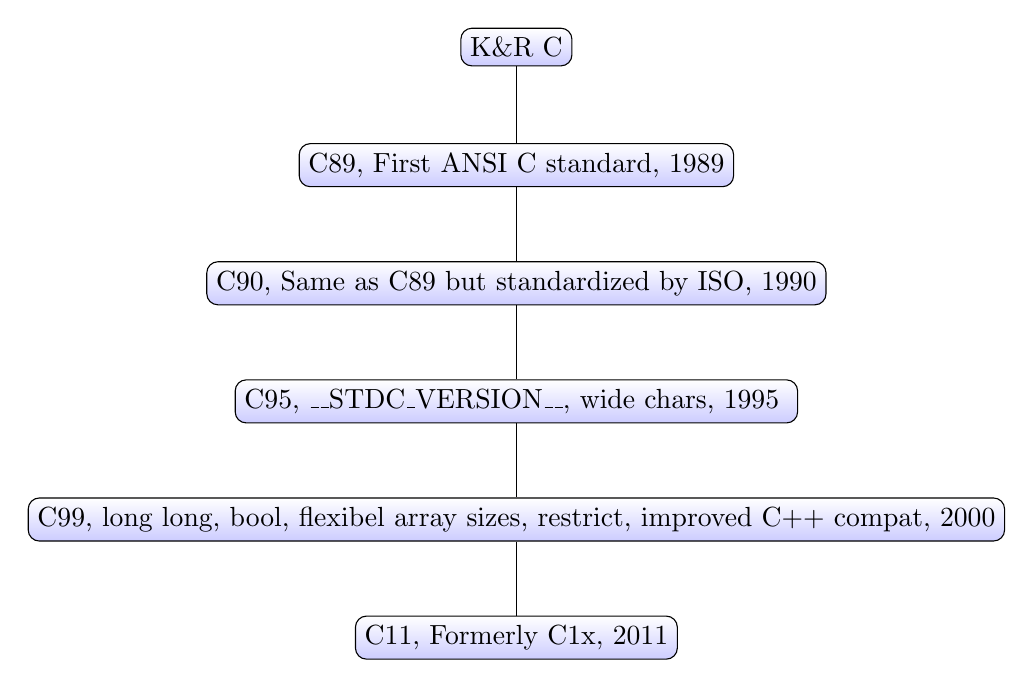
\begin{tikzpicture}[sibling distance=10em,
			every node/.style = {shape=rectangle, rounded corners,
				draw, align=center,
	top color=white, bottom color=blue!20}]]
	\node {K\&R C}
		child { node {C89, First ANSI C standard, 1989}
		child { node {C90, Same as C89 but standardized by ISO, 1990}
		child { node {C95, \_\_STDC\_VERSION\_\_, wide chars, 1995 }
		child { node {C99, long long, bool, flexibel array sizes, restrict, improved C++ compat, 2000}
		child { node {C11, Formerly C1x, 2011} } } } } };
\end{tikzpicture}
\end{frame}

\section{C11 - Not yet available}

\begin{frame}
	\frametitle{Features not yet available on GCC/GNU libc}
	\begin{center}
		\includegraphics[scale = 0.6]{more.ps}
	\end{center}
\end{frame}

\begin{frame}
	\frametitle{Bounds-checking interfaces (Annex K)}
	\begin{itemize}
		\item Security oriented changes, defined when \texttt{\_\_STDC\_LIB\_EXT1\_\_} is defined
		\item .. but there is no consensus that it actually helps
		\item Remove \texttt{\%n} from the \texttt{*printf*} variants
		\item Chop and zero fill when a runtime error happens on \texttt{gets\_s}, \texttt{strcpy\_s}, \texttt{strcat\_s}, ...
	\end{itemize}
\end{frame}

\begin{frame}
	\frametitle{Analyzability features (Annex L)}
	\begin{itemize}
		\item The program will help diagnose when undefined behaviors hit. For example
			\begin{itemize}
				\item An object is referred to outside of its lifetime
				\item The operand of the unary * operator has an invalid value
				\item The value of a pointer that refers to space deallocated by a call to the free or realloc function is used
			\end{itemize}
		\item GCC has partial support via ubsan: shifts and integer overflow
	\end{itemize}
\end{frame}

\begin{frame}
	\frametitle{Analyzability features (Annex L)}
	\texttt{integer\_overflow.c}
\end{frame}

\begin{frame}
	\frametitle{Threading}
	\texttt{<threads.h>} is essentially a standardization of operations
	on threads. It sounds like nobody is interested in
	writing a wrapper around \texttt{pthread} for now.
\end{frame}

\section{C11 - Mildly impressive features}

\begin{frame}
	\frametitle{Mildly impressive features}
	\begin{center}
		\includegraphics[scale = 0.6]{unimpressed-dog.ps}
	\end{center}
\end{frame}

\begin{frame}
	\frametitle{Mildly impressive features}
	\begin{itemize}
		\item Alignment specification \texttt{\_Alignas}, \texttt{\_Alignof}, \texttt{aligned\_alloc}. GCC's \texttt{align} attribute and \texttt{posix\_memalign} were used instead.
		\item The \texttt{\_Noreturn} function specifier, GCC has had a \texttt{noreturn} attribute for a while
		\item \texttt{quick\_exit} for when exit fails
		\item Macros for complex (in the mathematical sense) values
		\item An exclusive create-and-open mode for fopen
		\item Improved Unicode support
		\item \texttt{\_\_thread} standardized as \texttt{\_Thread\_local}
	\end{itemize}
\end{frame}

\begin{frame}
	\frametitle{Analyzability features (Annex L)}
	\texttt{unicode.c}
\end{frame}

\section{C11 - Cool features}

\begin{frame}
	\frametitle{Cool features}
	\begin{center}
		\includegraphics[scale = 0.18]{lama.ps}
	\end{center}
\end{frame}


\begin{frame}[fragile]
	\frametitle{Static assertions}
	\par The problem:
	\begin{lstlisting}
void workflow_core_list_init(void)
{
   XASSERTN(sizeof(struct workflow_core_list_ctx) <= WF_FUNCTION_STORAGE);
}
	\end{lstlisting}
	\pause
	\par Checking that the storage size is available is done at
	runtime, but all the information is available at compile time.
\end{frame}

\begin{frame}
	\frametitle{Static assertions}
	\texttt{static\_assertions.c}
\end{frame}

\begin{frame}[fragile]
	\frametitle{Anonymous structures and unions}
	\par The problem:
	\begin{lstlisting}
struct value {
	[...]
        union {
                int *i; 
                bool *b; 
                double *d; 
                char **t;
                void **c;
        } value;
	[...]
};
	\end{lstlisting}
	\par This can improve readability sometimes by not forcing the
	     programmer to specify a name to access to a union member.
\end{frame}

\begin{frame}[fragile]
	\frametitle{Generics}
	\begin{itemize}
	\item A switch/case on a type
	\item Is evaluated at compile time, after the pre-processor has run
	\end{itemize}
\end{frame}

\begin{frame}
	\frametitle{Generics}
	\texttt{generics*.c}
\end{frame}

\begin{frame}[fragile]
	\frametitle{Atomics}
	\begin{itemize}
		\item An ambitious change, also applies to composite types. \textit{a la} Java \texttt{volatile}
		\item \texttt{\_Atomic} type qualifier
		\item In gcc, atomic calls are implemented via libatomic
			\begin{lstlisting}
_Atomic int counter;
_Atomic struct { char c[512]; } my_struct;
			\end{lstlisting}
		\item Explicit memory models, default to sequential consistency (costly memory fences)
	\end{itemize}
\end{frame}

\begin{frame}[fragile]
	\frametitle{Atomics - basic types}
	\begin{itemize}
	\item \texttt{<stdatomic.h>} defines basic atomic types, like \texttt{atomic\_int}, \texttt{atomic\_long} and \texttt{atomic\_ullong}
	\item They \textit{might} be implemented with mutexes, but with gcc 5.2,  x86-64 they are lock free. This can be tested via the \texttt{ATOMIC\_INT\_LOCK\_FREE}, \texttt{ATOMIC\_LONG\_LOCK\_FREE}, ... macros
	\end{itemize}
\end{frame}


\begin{frame}[fragile]
	\frametitle{Atomics}
	\begin{itemize}
	\item \texttt{memory\_order} defines all possible memory models
	\begin{lstlisting}
enum memory_order {
	memory_order_relaxed,
	memory_order_consume,
	memory_order_acquire,
	memory_order_release,
	memory_order_acq_rel,
	memory_order_seq_cst, // the default
};
i = atomic_load_explicit(&atomic_counter, memory_order_relaxed);
j = atomic_load(&atomic_counter, memory_order_relaxed);
	\end{lstlisting}
	\item atomic \texttt{load}s and \texttt{store}s can take a memory ordering hint
	\end{itemize}
\end{frame}

\begin{frame}[fragile]
	\frametitle{Faster increments}
	\par Problem: increment a counter atomically 
	\begin{center}
		
\includegraphics[scale = 0.6]{knife.ps}
	\end{center}
\end{frame}



\begin{frame}[fragile]
	\frametitle{Faster increments}
	\begin{center}
		\texttt{concurrency.c}
	\end{center}
\end{frame}


\section{Compiling gateway with -std=c11}
\begin{frame}[fragile]
	\frametitle{gcc support table}
	\begin{center}
		\adjustbox{max height=\dimexpr\textheight-5.5cm\relax,
			           max width=\textwidth}{
		\begin{tabular}{rr}
			-std=c1x & GCC 4.6 \\
			-std=c11 & GCC 4.7 \\
			\_\_STDC\_VERSION\_\_ == 201112L & GCC 4.7 \\
			\_Alignas, \_Alignof, max\_align\_t, stdalign.h & GCC 4.7 \\
			\textbf{\_Atomic, stdatomic.h} & \textbf{GCC 4.9} \\
			\textbf{\_Generic} & \textbf{GCC 4.9} \\
			\_Noreturn, stdnoreturn.h & GCC 4.7 \\
			\textbf{\_Static\_assert} & \textbf{GCC 4.6} \\
			\_Thread\_local & GCC 4.9 \\
			Anonymous struct and union & GCC 4.6 \\
			Typedef redefinition & GCC 4.6 \\
			New macros in float.h & GCC 4.6 \\
			Macros for Complex values & GCC 4.7 + Library issue (glibc 2.16) \\
			Unicode strings & GCC 4.7 \\
			uchar.h & Library issue (glibc 2.16) \\
			static\_assert in assert.h & Library issue (glibc 2.16) \\
			Remove gets & Library issue (glibc 2.16) \\
			struct timespec, timespec\_get & Library issue (glibc 2.16) \\
			at\_quick\_exit, quick\_exit & Library issue (glibc 2.16) \\
			aligned\_alloc & Library issue (glibc 2.16) \\
			fopen mode "x" & Library issue (glibc 2.x) \\
			Analyzability (Annex L) [Optional] & - \\
			Bounds-checking (Annex K) [Optional] & Library issue (not implemented) \\
			Threading [Optional] & Library issue (not implemented) \\
	\end{tabular} }
	\end{center}
\end{frame}

\begin{frame}[fragile]
	\frametitle{The GCCs we use}
	\begin{center}
		\adjustbox{max height=\dimexpr\textheight-5.5cm\relax,
			           max width=\textwidth}{
		\begin{tabular}{rr}
		RHEL 5 (4.4) & 4.1.2 \\
		RHEL 6 & 4.4.5 \\
		RHEL 7 & 4.8.2 \\
		Ubuntu 10 & 4.6.3 \\
		Ubuntu 12 & 4.2.4 \\
		Ubuntu 14 & 4.8.2 \\
	\end{tabular} }
	\end{center}
\end{frame}



\section{Q\&A}
\begin{frame}
  \frametitle{Q\&A}
Questions
\end{frame}

\end{document}
